\documentclass[10pt]{beamer}	% Is better for some Windows user.
%
\usepackage{pict2e}
\usepackage{tikz}
\usepackage[ngerman]{babel} % Pakete laden
\usepackage[utf8]{inputenc}
\usepackage[T1]{fontenc}
\usepackage{graphicx, xcolor}
% \usepackage{BeamerColor}
\usepackage{tikz, amsfonts, amsmath}
\usetheme{Goettingen}
% \usecolortheme[named=darkgray]{structure}
\def\UDM{ % untere Dreiecks-Matrix
\mbox{
\setlength{\unitlength}{9pt}
\begin{picture}(1,1)
\put(0,1){\line(1,0){1}}
\put(1,0){\line(0,1){1}}
\put(0,1){\line(1,-1){1}}
\end{picture}
}}
\title{Homogenization of Solid Oxide Fuel Cell}
\author{Janna Puderbach}
% \input{docinfo}				% Edit here author informations.
% \input{header}
% \input{titlepage}
% \input{headingsandfooter}
\usepackage{algorithm2e}
\begin{document}
    \addtocounter{framenumber}{-1}	% Exclude page from pagecounter.
	\begin{frame}[plain]
		\titlepage
	\end{frame}
	%
	%\setcounter{framenumber}{0}
	\frame{
		\frametitle{Content}
		\tableofcontents
	}



	
	\section{Model}
	\begin{frame}
	\begin{figure}
		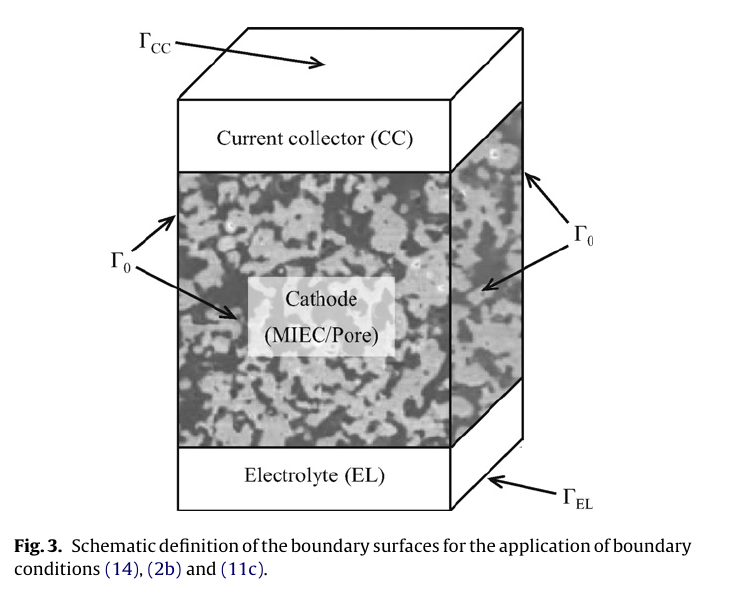
\includegraphics[scale=0.125]{SOFC_picture_3D.png}
% 	\end{figure}
% 	\begin{figure}
	\begin{tikzpicture}
%microscopic structure
\draw (1/64,1/64) -- (1/64,131/64) -- (131/64,131/64) -- (131/64,1/64) -- (1/64,1/64);

  \foreach \x in {1,...,32}
  {
    \foreach \y in {1,...,32}
    {
		\fill[gray] (\x/16,\y/16) circle (0.2mm);
	}
  }
%   \node at (2.5,2.5){\small{microscopic problem}};
	\end{tikzpicture}
% 	\caption{Microscopic problem }
	\end{figure}
	\begin{align*}
		\nabla \cdot ( D_V\nabla u) &= f \quad  &\text{in} \Omega 		\\	% In Omega
		D_V \nabla u \cdot \nu &= k(u - \bar u)  \quad  &\text{on} \Gamma	\\	% Robin on Holes
		u = 0  ,\quad u &= 1  \quad &\text{on} \partial\Omega_D 				\\	% Dirichlet
		\nabla u \cdot \nu &= 0  \quad &\text{on} \partial\Omega_N							% Neumann 0
	\end{align*}
		\end{frame}
	\section{Homogenization}
% 	\begin{frame}
% 		Model -> Microscopic -> Homogenization -> Cell Problem -> Diffusion-tensor -> Macroscopic 
% 	\end{frame}

	\begin{frame}
	\begin{figure}
	\begin{tikzpicture}	
		% periodicity cell
	\draw (4.25,0.25) -- (4.25,2.25) -- (6.25,2.25) -- (6.25,0.25) -- (4.25,0.25);
	\fill[gray] (5.25,1.25) circle (5mm);
	\node at (4.75,1.75) {$\Omega_2$};
	\node at (5.25,1.25) {$\Omega_1$};
	\node at (6.75,0.25) {$\Pi$};
	\draw[|-|] (4.25,0) -- (6.25,0);
	\node  at (5.25,-0.25){$l$};
	
	 \fill [gray] (6.25,0.25) rectangle (8.25,2.25);
	 \draw (6.25,0.25) -- (6.25,2.25) -- (8.25,2.25) -- (8.25,0.25) -- (6.25,0.25);
		
	\end{tikzpicture}
	\end{figure}
	\end{frame}
	
	\begin{frame}{Homogenization}
		\begin{itemize}
% 			\item Seperate macroscale and microscale $u(x) = u(x,y) $ with $y= x/\varepsilon$
% 			\item Ansatz: $u(x,y) = u_0(x,y) + \varepsilon u_1(x,y) + \varepsilon^2 u_2(x,y) + ...$\\
% 					$\nabla = \nabla_x + \frac{1}{\varepsilon}\nabla_y$
			\item Solve cell problem 
			\item Compute effective diffusion tensor
			\item Solve macroscopic/homogenized problem
		\end{itemize}
	\end{frame}
% 	\section{Microscopic Problem}
% 	
% 	\section{Cell Problem}
% 	
% 	\section{Macroscopic Problem}
% 	
% 	\section{Homogenization of the boundary condition}
	
	\section{Outlook}
	\begin{frame}
	\begin{itemize}
		\item Considering and implementation second material
		\item Comparison of the microscopic and the macroscopic/homogenized solution
		\item Extend to the 3D model
	\end{itemize}
	\end{frame}

%\section{Introduction}
% 
% \begin{frame}{Introduction} %Motivation
% Given a composite material %Bild
% \begin{figure}
% \begin{tikzpicture}
% %microscopic structure
% \draw (0.25,0.25) -- (0.25,2.25) -- (2.25,2.25) -- (2.25,0.25) -- (0.25,0.25);
% 
%   \foreach \x in {1,...,4}
%   {
%     \foreach \y in {1,...,4}
%     {
% 		\fill[gray] (\x/2,\y/2) circle (1mm);
% 	}
%   }
% 		
% 	\draw[dashed] (1.75,1.75) -- (1.75,1.25) -- (1.25,1.25) -- (1.25,1.75) -- (1.75,1.75);
% 	
% 	\draw[|-|] (0.25,0) -- (2.25,0);
% 	\node at (1.25,-0.25){$L$};
% 	
% 	\draw[|-|] (2.5,1.75) -- (2.5,1.25);
% 	\node at (2.75,1.5){$l$};
% 	
% 	\node at (2.75,0.25){$\Omega$};
% 	
% % 	\draw[out=30, in=30] (1.75,1.75) to (4,25,2.25) ;
% 	
% % periodicity cell
% \draw (4.25,0.25) -- (4.25,2.25) -- (6.25,2.25) -- (6.25,0.25) -- (4.25,0.25);
% \fill[gray] (5.25,1.25) circle (5mm);
% \node at (4.75,1.75) {$\Omega_2$};
% \node at (5.25,1.25) {$\Omega_1$};
% \node at (6.75,0.25) {$\Pi$};
% \draw[|-|] (4.25,0) -- (6.25,0);
% \node  at (5.25,-0.25){$l$};
% 	
% \end{tikzpicture}
% \end{figure}
% \begin{itemize}
% \item $\Omega$ - domain with macroscale $L$
% \item $\Pi$ - periodic cell with microscale $l$
% \item Assume $\varepsilon = \frac{l}{L} \ll 1$
% \item Solve with FEM too expensive (very fine mesh)
% 
% 
% \end{itemize}
% % \textbf{microscopic scale}
% % \begin{itemize}
% % \item fine scale of inhomogeneous part
% % \item too expensive to solve with FEM
% % \end{itemize}
% % \textbf{macroscopic scale}
% % \begin{itemize}
% % \item Consider the material as homogeneous
% % \item easy to solve
% % \end{itemize}
% \end{frame}
% 
% 
% \begin{frame}{Homogenization}
% \begin{itemize}
% \item Homogenization: $\varepsilon \to 0$
% \end{itemize}
% \begin{figure}
% \begin{tikzpicture}
% %first domain
% \draw (0.25,0.25) -- (0.25,2.25) -- (2.25,2.25) -- (2.25,0.25) -- (0.25,0.25);
% 
%   \foreach \x in {1,...,4}
%   {
%     \foreach \y in {1,...,4}
%     {
% 		\fill[gray] (\x/2,\y/2) circle (1mm);
% 	}
%   }
% 		
% % 	\draw[dashed] (1.75,1.75) -- (1.75,1.25) -- (1.25,1.25) -- (1.25,1.75) -- (1.75,1.75);
% % 	
% % 	\draw[|-|] (0.25,0) -- (2.25,0);
% % 	\node at (1.25,-0.25){$L$};
% % 	
% % 	\draw[|-|] (2.5,1.75) -- (2.5,1.25);
% % 	\node at (2.75,1.5){$l$};
% % 	
% % 	\node at (2.75,0.25){$\Omega$};
% 	
% 	
% 	%second domain
% 	\draw (3.25,0.25) -- (3.25,2.25) -- (5.25,2.25) -- (5.25,0.25) -- (3.25,0.25);
% 
%   \foreach \x in {1,...,8}
%   {
%     \foreach \y in {1,...,8}
%     {
% 		\fill[gray] (\x/4+3.125,\y/4+0.125) circle (0.5mm);
% 	}
%   }
% % 		
% % 	\draw[dashed] (1.75,1.75) -- (1.75,1.25) -- (1.25,1.25) -- (1.25,1.75) -- (1.75,1.75);
% % 	
% % 	\draw[|-|] (0.25,0) -- (2.25,0);
% % 	\node at (1.25,-0.25){$L$};
% % 	
% % 	\draw[|-|] (2.5,1.75) -- (2.5,1.25);
% % 	\node at (2.75,1.5){$l$};
% % 	
% % 	\node at (2.75,0.25){$\Omega$};
% 	
% 	%third domain
% % 	\draw (8.25,0.25) -- (8.25,2.25) -- (10.25,2.25) -- (10.25,0.25) -- (8.25,0.25);
% 	 \fill [gray] (6.25,0.25) rectangle (8.25,2.25);
% 	 \draw (6.25,0.25) -- (6.25,2.25) -- (8.25,2.25) -- (8.25,0.25) -- (6.25,0.25);
% 	
% \end{tikzpicture}
% \end{figure}
% \end{frame}
% 
% % %Example
% \section{Example}
% \begin{frame}{Example (Diffusion Problem)}
% 
% \begin{figure}
% \begin{tikzpicture}
% 
% % periodicity cell
% \draw (4.25,0.25) -- (4.25,2.25) -- (6.25,2.25) -- (6.25,0.25) -- (4.25,0.25);
% \fill[gray] (5.25,1.25) circle (5mm);
% \node at (4.75,1.75) {$\sigma_2$};
% \node at (5.25,1.25) {$\sigma_1$};
% \node at (6.75,0.25) {$\Pi$};
% \draw[|-|] (4.25,0) -- (6.25,0);
% \node  at (5.25,-0.25){$l$};
% 	
% \end{tikzpicture}
% \end{figure}
% \begin{align*}
% - \operatorname{div} \only<1>{(\sigma(x) \nabla u) &= g(x), \quad & x \in \Omega} \only<2>{(\sigma(x/\varepsilon) \nabla u_{\varepsilon}) &= g(x), \quad & x \in \Omega} \\
% \only<1> {u &= 0 , \quad & x \in \partial \Omega} \only<2>{u_\varepsilon &= 0 , \quad & x \in \partial \Omega }
% \end{align*}
% Diffusion Tensor rapidly oscillates
% \begin{align*}
% \sigma(x) &= \begin{cases} \sigma_1 , \quad x\in \Omega_1\\ \sigma_2, \quad 
% x\in \Omega_2 \end{cases}
% \end{align*}
% 
% % \begin{tikzpicture}
% % \draw  ;
% % \end{tikzpicture}
% \end{frame}
% %
% 
% % %formal asymptotic expansion
% \begin{frame}{Formal Asymptotic Expansion}
% Ansatz:
% \begin{align*}
% % \only<1>{u_{\varepsilon} (x) = u_0(x,\frac{x}{\varepsilon}) + \varepsilon u_1(x,\frac{x}{\varepsilon}) + \varepsilon^2 u_2(x,\frac{x}{\varepsilon}) + ...}
% u_{\varepsilon}(x) = u_0(x,y) + \varepsilon u_1(x,y) + \varepsilon^2 u_2(x,y) + ...
% \end{align*}
% \begin{itemize}
% \item with $u_\varepsilon$ is $\Pi$-periodic in $y = \frac{x}{\varepsilon}$ 
% \item  $x$ - slow variable and $y$ - fast variable
% \item Consider $x$ and $y$ as independent variables
% \end{itemize}
% With chain rule for $\nabla$:
% \begin{align*}
% \nabla = \nabla_x + \frac{1}{\varepsilon} \nabla_y
% \end{align*}
% \end{frame}
% 
% \begin{frame}
% \begin{align*}
% &-\varepsilon^{-2}\operatorname{div}_y(\sigma(y)\nabla_y u_0(x,y))\\
% &-\varepsilon^{-1}[\operatorname{div}_y(\sigma(y)\nabla_y u_1(x,y)) + \operatorname{div}_y(\sigma(y)\nabla_x u_0(x,y)\\ &+ \operatorname{div}_x(\sigma(y)\nabla_y u_0(x,y))]\\
% &-\varepsilon^0 [\operatorname{div}_y(\sigma(y)\nabla_y u_2(x,y)\sigma(y)\nabla_x u_1(x,y)) \\&+ \operatorname{div}_x(\sigma(y)\nabla_y u_1(x,y) +  \operatorname{div}_x(\sigma(y)\nabla_x u_0(x,y)]\\
% &-\varepsilon^1 ... =g(x)
% \end{align*}
% \end{frame}
% 
% \section{Homogenized Problem}
% \begin{frame}{Homogenized Problem}
% 
% \begin{align*}
% \only<1>{-\operatorname{div} (\hat \sigma \nabla u_0) &= g(x), \quad &x \in \Omega \\
% u_0 &=0, \quad &x \in \partial \Omega}
% % \only<2>{(\hat \sigma \nabla u_0, \nabla \phi) = (g,\phi) , \quad \forall \phi}
% \end{align*}
% \begin{itemize}
% \item $\hat \sigma $ - homogenized diffusion tensor
% \begin{align*}
% \hat \sigma_{i,j} = \frac{1}{|\Pi|} \int_{\Pi} (\sigma(y)(\nabla \chi_i + \boldsymbol e_i)) \cdot (\nabla \chi_j + \boldsymbol e_j) \operatorname d y
% \end{align*}
% \item $\boldsymbol e_i$ - unit vector
% \item $\chi_i$ - solution of the cell problem
% \end{itemize}
% \begin{align*}
% - \operatorname{div} \left[ \sigma(y)[\nabla \chi_i + \boldsymbol e_i ]\right] = 0 , \quad y \in \Pi
% \end{align*}
% \end{frame}
% \begin{frame}{Cell Problem}
% \begin{align*}
% - \operatorname{div} \left[ \sigma(y)[\nabla \chi_i + \boldsymbol e_i ]\right] = 0 , \quad y \in \Pi
% \end{align*}
% \begin{figure}
% \begin{tikzpicture}
% \draw[blue,thick]   (0,0) -- (2,0);
% \draw[blue,thick]   (2,2) -- (0,2);
% \draw[red,thick]    (0,2) -- (0,0);
% \draw[red,thick]    (2,0) -- (2,2);
% \draw[white] (0.5,1.5) circle (0.2cm) node[black]{$\sigma_1$};
% \draw[white] (1,1) circle (0.2cm) node[black]{$\Pi$};
% \fill[gray] (1,1) circle (0.5cm) node[white]{$\sigma_2$};
% \end{tikzpicture}
% % \caption{Unit cell}
% \end{figure}
% \begin{itemize}
% \item periodic boundary conditions
% % \item $\sigma$ defined with levelset-function
% \end{itemize}
% \end{frame}
% 
% \begin{frame}{Convergence}
% \textbf{Theorem}
% Let 
% $u_\varepsilon(x)$ be the solution of:
% \begin{align*}
% -\operatorname{div} (\sigma(\frac{x}{\varepsilon}) \nabla u_{\varepsilon}) &= g(x) , \quad & x \in \Omega\\
% u_{\varepsilon} &= 0, \quad &x \in \partial \Omega
% \end{align*}
% in a bounded domain $\Omega$. Then 
% \begin{align*}
% u_{\varepsilon} &\rightharpoonup u_0 &\text{ weakly in } &H^1_0(\Omega)\\
% \sigma_{\varepsilon}\nabla u_{\varepsilon} &\rightharpoonup \hat \sigma \nabla u_0 &\text{ weakly in } &L^2(\Omega)
% \end{align*}
% \end{frame}
% 
% 
% %
% 
% %
% \section{Two-Scale Convergence}
% %Two-scale convergence
% \begin{frame}{Two-Scale Convergence}
% 
% \textbf{Definition}
% \begin {itemize}
% \item Let $\{u_\varepsilon\}$ be a sequence of functions from $L^2(\Omega)$
% \item  $u_\varepsilon$ two-scale converges to a limit
% $u_0(x,y)\in L^2(\Omega \times \Pi)$
% \\
% \item if $\{u_\varepsilon\}$ is bounded in $L^2(\Omega)$ and
% \item for any function $\Psi(x,y)\in D(\Omega,C^\infty_{per}(\Pi))$ the following equality holds:
% \end{itemize}
% 
% \begin{align*}
% \lim_{\varepsilon \to 0} \int_
% {\Omega} u_\varepsilon (x) \Psi(x,\frac{x}{\varepsilon}) \operatorname d x = \int_{\Omega} \int_\Pi u_0(x,y) \Psi(x,y)\operatorname d y \operatorname d x
% \end{align*}
% 
% \begin{itemize}
% \item version of weak convergence
% \item strong convergence $\Rightarrow$ Two-scale convergence
% \item two-scale convergence $\Rightarrow$ weak convergence (but limits may differ)
% \end{itemize}
% \end{frame}
% 

% \begin{frame}
% \begin{itemize}
% \item microscopic problem
% \begin{itemize}
% \item very fine grid necessary to resolve the structure
% \end{itemize}
% \item Homogenized problem
% \begin{itemize}
% \item need to solve extra problem (cell problem)
% \end{itemize}
% \end{frame}
%\begin{frame}{Quellen}

%\end{frame}

% \begin{frame}
% \begin{center}
%     \begin{huge}
%     Vielen Dank für Ihre Aufmerksamkeit!\\[1,5cm]
%     Fragen?
%     \end{huge}
% \end{center}
%
% \end{frame}

\end{document}
